\documentclass[UTF8,fontset=fandol,zihao=-4]{ctexart}

\usepackage[a4paper,top=2.5cm,bottom=2.5cm,left=2.6cm,right=2.6cm]{geometry}
\usepackage{array}
\usepackage{booktabs}
\usepackage{longtable}
\usepackage{tabularx}
\usepackage{enumitem}
\usepackage{xcolor}
\usepackage{hyperref}
\usepackage{fancyhdr}
\usepackage{titlesec}
\usepackage{setspace}
\usepackage{listings}
\usepackage{graphicx}

\hypersetup{
  colorlinks=true,
  linkcolor=black,
  urlcolor=blue,
  citecolor=black
}

\pagestyle{fancy}
\fancyhf{}
\fancyhead[L]{基于 WebGL 的轻量化 3D 家居设计平台}
\fancyhead[R]{创新训练项目申请书}
\fancyfoot[C]{\thepage}
\renewcommand{\headrulewidth}{0.4pt}

\titleformat{\section}{\centering\Large\bfseries}{\chinese{section}、}{0pt}{}
\titleformat{\subsection}{\large\bfseries}{\thesubsection}{0.8em}{}
\titleformat{\subsubsection}{\normalsize\bfseries}{\thesubsubsection}{0.8em}{}

\setlist[itemize]{leftmargin=2em,itemsep=0.2em,topsep=0.2em}
\setlist[enumerate]{leftmargin=2.5em,itemsep=0.2em,topsep=0.2em}
\renewcommand{\arraystretch}{1.35}
\setlength{\tabcolsep}{4pt}
\setlength{\headheight}{15pt}
\setlength{\LTleft}{0pt}
\setlength{\LTright}{0pt}
\setlength{\parindent}{2em}
\setlength{\parskip}{0.25em}
\linespread{1.25}
\sloppy

\lstset{
  basicstyle=\ttfamily\small,
  breaklines=true,
  frame=single,
  columns=fullflexible,
  keepspaces=true
}

\graphicspath{{docs/plans/assets/}}

\newcolumntype{Y}{>{\raggedright\arraybackslash}X}
\newcolumntype{P}[1]{>{\raggedright\arraybackslash}p{#1}}

\begin{document}

\begin{titlepage}
  \centering
  \vspace*{2.5cm}
  {\zihao{1}\bfseries 大学生创新创业训练计划项目申请书\par}
  \vspace{2.2cm}
  {\zihao{2}\bfseries 基于 WebGL 的轻量化 3D 家居设计平台设计与实现\par}
  \vspace{1.5cm}
  {\zihao{3} 创新训练项目\par}
  \vfill
  \begin{tabular}{P{4cm}P{8cm}}
    申报学院： & 智能技术学部 \\
    项目负责人： & 刘宇航 \\
    指导教师： & 蒋文萍 \\
  \end{tabular}
  \vspace*{2cm}
\end{titlepage}

\tableofcontents
\newpage

\section{项目基本信息}

\begin{table}[h]
\centering
\begin{tabularx}{\textwidth}{P{3.2cm}Y}
\toprule
项目 & 内容 \\
\midrule
项目名称 & 基于 WebGL 的轻量化 3D 家居设计平台设计与实现 \\
项目类别 & 创新训练项目 \\
项目级别 & 国家级 \\
申报学院 & 智能技术学部 \\
项目负责人 & 刘宇航 \\
团队成员 & 黄灿斌、徐峥、陶锦昕、肖斯霖 \\
指导教师 & 蒋文萍 \\
申请经费 & 5000 元 \\
\bottomrule
\end{tabularx}
\end{table}

\section{立项依据}

\subsection{项目背景}

随着居民生活水平提升、租房改造和个性化家居布置需求增长，普通消费者对室内空间可视化设计工具的需求日益明显。很多用户在购买家具、改造房间或规划装修前，希望先在屏幕中直观看到空间布局、家具尺寸和整体效果，从而降低试错成本。

目前市场上的室内设计工具大致分为两类：一类是 AutoCAD、SketchUp、3ds Max 等专业软件，功能强但学习成本高，对普通消费者不友好；另一类是酷家乐、三维家等偏家装行业的设计平台，功能完整但更面向设计师、家装公司和商业场景。面向普通用户的免安装、轻量化、可快速上手的 Web 端 3D 家居设计工具仍然不足。

WebGL、Three.js、React Three Fiber 等技术的发展，使复杂 3D 交互逐步从桌面软件迁移到浏览器中成为可能。浏览器端工具具备零安装、跨平台、易分享、易部署的优势，适合作为面向大众的轻量化设计入口。因此，本项目拟研究并实现一款基于 WebGL 的轻量化 3D 家居设计平台，为普通用户提供房间搭建、家具布置、场景保存与效果预览能力。

\subsection{研究意义}

本项目具有以下研究与实践意义：

\begin{enumerate}
  \item \textbf{降低普通用户的 3D 设计门槛。} 项目将复杂建模流程拆解为“建筑结构编辑”和“家具布置装饰”两个阶段，使没有专业建模经验的用户也能完成基础户型搭建和家居布局。
  \item \textbf{探索浏览器端住宅空间编辑内核。} 项目围绕墙体绘制、顶点连接、区域生成、拓扑修复、墙体网格生成等问题，研究适合 Web 端实时交互的轻量化建筑编辑模型。
  \item \textbf{验证 Web 3D 场景管理与持久化方案。} 项目基于 React、Three.js、Zustand 和 IndexedDB，探索浏览器端 3D 场景状态管理、模型资产加载、本地保存与恢复机制。
  \item \textbf{形成可持续扩展的创新训练成果。} 项目已有可运行原型和较完整的工程基础，后续可继续拓展门窗、材质、测量、导出、分享等能力，为论文、软著和竞赛成果提供支撑。
\end{enumerate}

\subsection{国内外现状分析}

国外已有 Planner 5D、Floorplanner、HomeByMe、SketchUp Web 等 Web 端或云端设计工具。这些产品在可视化、模板化和在线编辑方面积累较多，但部分工具模型库封闭、免费能力有限，或者仍偏向专业建模与复杂空间设计。

国内以酷家乐、三维家、躺平设计家等平台为代表，主要服务家装公司、设计师和商业转化场景，具备强大的渲染与商品库能力，但普通消费者在轻量使用、自定义模型导入、开源可扩展等方面仍有需求空间。

从技术角度看，React Three Fiber、Three.js、glTF/GLB、IndexedDB 等技术已经成熟，但将其组合为一个稳定的浏览器端住宅空间编辑工具，仍需要解决墙体拓扑、区域识别、3D 交互反馈、模型加载性能、本地持久化可靠性等具体工程问题。本项目的创新点正是在现有 Web 3D 技术基础上，面向家居设计这一具体应用场景进行系统化集成与优化。

\section{项目目标与研究内容}

\subsection{总体目标}

本项目拟设计并实现一款完全运行在浏览器中的轻量化 3D 家居设计平台。用户无需安装专业软件，即可完成房间结构绘制、墙体高度调整、家具模型上传与摆放、场景保存和效果预览等操作。

项目目标包括：

\begin{enumerate}
  \item 构建浏览器端 3D 家居设计原型系统，实现从空白场景到室内布局方案的核心流程。
  \item 研究适合 Web 端实时交互的住宅建筑编辑内核，支持墙体、顶点、区域等基础空间对象。
  \item 实现建筑编辑与家具布置分离的两阶段交互范式，降低用户认知负担。
  \item 建立 GLB 模型资产加载、管理与上传机制，支持用户自定义家具模型。
  \item 实现场景本地持久化与基础后端资产服务，为后续云端同步、分享和模型库建设预留接口。
  \item 形成可演示 Demo、技术文档、测试报告、论文或软件著作权等项目成果。
\end{enumerate}

\subsection{主要研究内容}

\subsubsection{浏览器端建筑编辑内核}

项目将房间结构抽象为顶点、墙体、区域等对象，研究墙体绘制、端点吸附、墙体相交、区域闭合、拓扑修复和区域重建等问题。通过稳定的建筑编辑内核，使用户能够在浏览器中绘制和调整住宅平面结构。

当前项目仓库已具备 architecture 相关模块，包括 topology、geometry、domain、editing 等分层结构。后续研究将继续完善墙体连接规则、区域身份稳定、墙体网格生成和编辑反馈机制。

\subsubsection{建造与装饰两阶段交互范式}

为降低普通用户使用 3D 工具的难度，项目将设计流程拆解为两个阶段：

\begin{itemize}
  \item \textbf{建造阶段：} 用户主要完成房间轮廓、墙体结构、区域划分等操作。
  \item \textbf{装饰阶段：} 用户主要完成家具选择、模型上传、放置、移动、旋转和缩放等操作。
\end{itemize}

这种分阶段设计能够减少工具复杂度，使用户先建立空间结构，再进行室内布置，符合实际装修设计流程。

\subsubsection{WebGL 3D 场景渲染与交互}

项目基于 Three.js 和 React Three Fiber 实现 3D 场景渲染，研究墙体、地面、家具模型和辅助交互元素的渲染方式。针对室内观察时墙体遮挡的问题，项目将设计墙体透明切换、屋顶显示控制、第一人称漫游和俯视编辑等交互方式。

项目还将关注浏览器端性能优化，包括按需加载模型、减少不必要的渲染更新、优化状态订阅、控制模型复杂度等，以保证普通设备上的交互流畅性。

\subsubsection{家具模型资产管理}

项目支持 GLB 格式家具模型的上传、浏览、放置和变换。前端负责模型选择、预览和场景放置，后端资产服务负责模型文件、缩略图、分类信息和元数据管理。

该模块将研究用户自定义模型导入、模型资源管理、缩略图生成、模型文件大小限制和模型加载失败处理等问题，为开放素材库和社区扩展奠定基础。

\subsubsection{场景状态管理与本地持久化}

项目使用 Zustand 管理编辑器状态，并通过 IndexedDB 或本地存储机制保存用户设计内容。研究内容包括场景数据结构设计、家具变换信息保存、建筑结构保存、自动恢复、版本迁移和异常恢复等。

持久化能力能够避免用户误关闭页面导致设计丢失，也为后续跨设备同步和分享链接功能提供数据基础。

\subsection{拟解决的关键问题}

\begin{enumerate}
  \item \textbf{浏览器端建筑拓扑稳定性问题。} 墙体绘制和编辑过程中会出现端点重合、T 字连接、十字交叉、闭合区域变化等情况。项目需要设计稳定的拓扑修复和区域重建算法，保证编辑结果可靠。
  \item \textbf{普通用户低门槛 3D 操作问题。} 传统 3D 软件交互复杂，普通用户难以理解坐标轴、视角、模型变换等概念。项目需要通过分阶段模式、可视化提示、拖拽操作和快捷反馈降低使用门槛。
  \item \textbf{室内空间遮挡与可视化问题。} 3D 房间中墙体和屋顶会遮挡内部家具，影响观察和编辑。项目需要设计墙体透明、局部隐藏、第一人称漫游和俯视切换等交互方案。
  \item \textbf{GLB 模型加载与性能问题。} 用户上传的家具模型可能文件较大、面数较高，导致浏览器卡顿或加载失败。项目需要研究模型资源管理、加载状态反馈和性能约束机制。
  \item \textbf{本地持久化可靠性问题。} 设计数据涉及房间结构、家具对象、模型资产和用户交互状态。项目需要设计清晰的数据结构，保证保存、恢复和后续版本升级的可靠性。
\end{enumerate}

\section{项目特色与创新点}

\subsection{面向普通消费者的零安装 Web 3D 家居设计工具}

项目区别于专业建模软件和偏 B 端的家装设计平台，定位于普通消费者的轻量化家居设计需求。用户通过浏览器即可使用，无需安装客户端或掌握复杂建模知识。

\subsection{建筑编辑与家具布置分离的交互模式}

项目将空间结构搭建和家具摆放拆分为两个阶段，避免用户在同一界面中面对过多工具和操作概念。该模式更符合普通用户“先定房间，再摆家具”的认知路径。

\subsection{面向 Web 端实时编辑的住宅空间数据模型}

项目以顶点、墙体、区域等对象构建轻量化建筑编辑模型，并结合拓扑修复、区域识别和墙体网格生成，实现浏览器端可交互的住宅空间编辑能力。

\subsection{开放的 GLB 模型导入与资产管理机制}

项目支持用户上传自定义 GLB 家具模型，避免完全依赖封闭素材库。后续可继续扩展模型分类、在线素材库、共享模型和模型质量检测等功能。

\subsection{工程化验证充分，具备持续迭代基础}

项目仓库已形成 React 19、TypeScript、Vite、Three.js、React Three Fiber、Zustand、Vitest、Playwright 等技术栈组合。当前 src 目录约 129 个文件，src、tests、server 下约 146 个 TypeScript/JavaScript 文件，代码量约 1.4 万行，并包含约 47 个测试相关文件，具备继续研发和验证的工程基础。

\section{研究方案与技术路线}

\subsection{总体技术路线}

项目采用“前端浏览器编辑器 + 本地持久化 + 后端资产服务”的技术路线：

\begin{lstlisting}
用户浏览器
  |
  |-- React + TypeScript 前端界面
  |-- React Three Fiber / Three.js 3D 渲染层
  |-- Zustand 编辑状态管理
  |-- IndexedDB 本地持久化
  |
后端资产服务
  |
  |-- GLB 模型上传
  |-- 缩略图与元数据管理
  |-- 模型分类与资产接口
\end{lstlisting}

结合当前最新的 \texttt{professional-editing-ux} worktree，项目已经从基础房间原型推进到专业编辑体验阶段：新增 \texttt{EditHandle} 数据模型、顶点拖拽与吸附、墙体数值输入、尺寸标注、选中/悬停视觉反馈和编辑状态提示等能力。依据长期路线图，项目后续将围绕“V3 稳定建筑内核、V4 完善编辑体验、V5 引入住宅语义、V6 做展示交付”的顺序推进。

\begin{figure}[htbp]
  \centering
  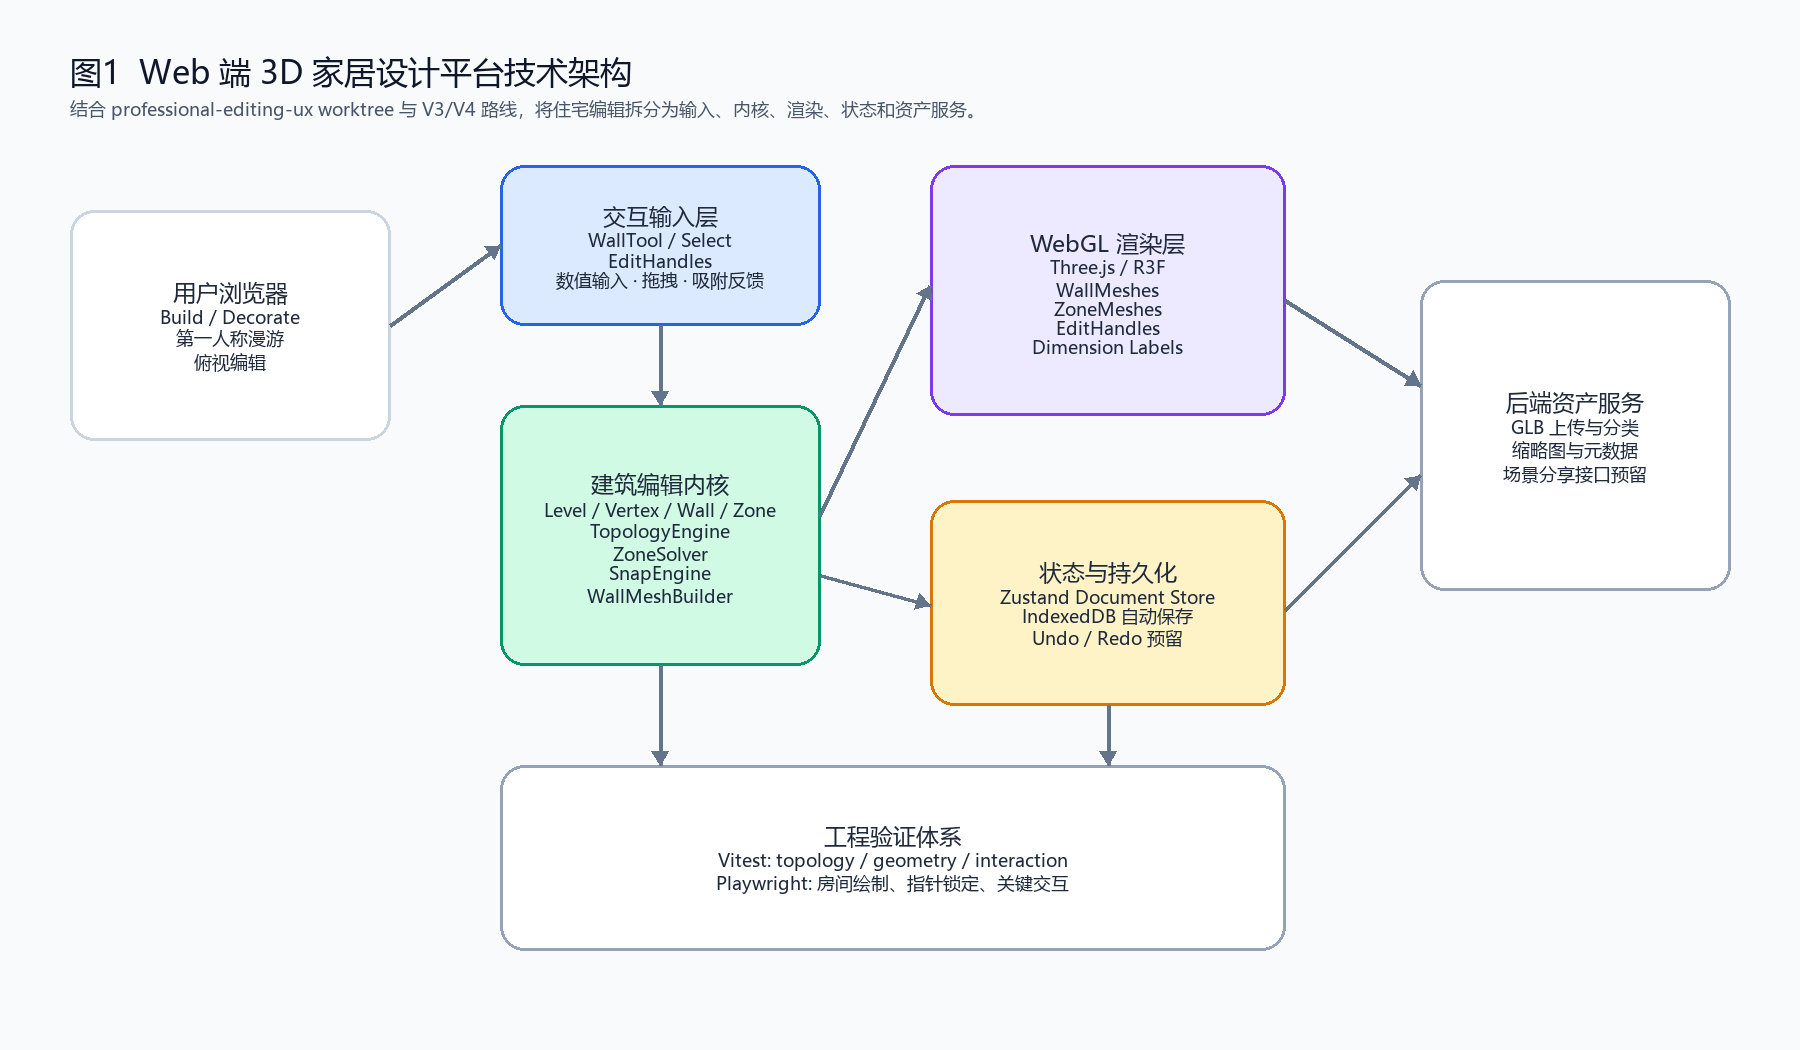
\includegraphics[width=\textwidth]{technical-architecture.png}
  \caption{Web 端 3D 家居设计平台技术架构}
\end{figure}

\subsection{技术选型}

\begin{longtable}{P{3cm}P{4.3cm}P{7cm}}
\toprule
模块 & 技术方案 & 作用 \\
\midrule
\endfirsthead
\toprule
模块 & 技术方案 & 作用 \\
\midrule
\endhead
前端框架 & React 19 + TypeScript & 构建类型安全的组件化 Web 应用 \\
构建工具 & Vite & 提供快速开发与生产构建能力 \\
3D 渲染 & Three.js + React Three Fiber & 实现浏览器端 3D 场景、模型和交互 \\
交互组件 & Drei / TransformControls & 支持模型移动、旋转、缩放等操作 \\
状态管理 & Zustand & 管理建筑文档、家具对象、UI 状态 \\
持久化 & IndexedDB / 本地存储 & 保存和恢复用户设计场景 \\
后端服务 & Node.js / TypeScript & 管理模型资产、分类、缩略图等 \\
测试体系 & Vitest + Playwright & 覆盖单元测试、集成测试和端到端流程 \\
\bottomrule
\end{longtable}

\subsection{研究方法}

\begin{enumerate}
  \item \textbf{需求调研法。} 通过竞品分析和目标用户访谈，梳理普通消费者在家居设计中的主要需求和操作痛点。
  \item \textbf{原型迭代法。} 基于已有项目原型进行增量开发，通过阶段性版本验证建筑编辑、家具布置、保存恢复等核心流程。
  \item \textbf{模块化工程设计法。} 将建筑编辑、几何生成、渲染显示、状态管理、资产服务等模块分层设计，降低耦合度，提高可维护性。
  \item \textbf{测试驱动与回归验证法。} 对墙体吸附、区域重建、模型变换、持久化和关键用户流程建立自动化测试，减少迭代过程中的功能回退。
  \item \textbf{用户体验评估法。} 邀请真实用户完成指定设计任务，记录完成时间、错误率、主观满意度和反馈意见，用于优化交互流程。
\end{enumerate}

\section{项目实施计划}

\begin{longtable}{P{2.4cm}P{3.2cm}P{5.4cm}P{4.1cm}}
\toprule
阶段 & 时间 & 主要任务 & 阶段成果 \\
\midrule
\endfirsthead
\toprule
阶段 & 时间 & 主要任务 & 阶段成果 \\
\midrule
\endhead
第一阶段：需求调研与方案完善 & 2026 年 3 月至 4 月 & 完成竞品分析、用户需求调研、技术路线确认，整理已有原型功能 & 调研报告、需求文档、技术方案 \\
第二阶段：建筑编辑内核完善 & 2026 年 5 月至 6 月 & 完善 V3 建筑编辑内核，稳定 Wall/Vertex/Zone identity，补强拓扑修复、Zone 重建、墙体 mesh 和回归测试 & 建筑编辑核心 Demo、单元测试 \\
第三阶段：编辑体验与 3D 交互优化 & 2026 年 7 月至 8 月 & 推进 V4 专业编辑体验，实现 EditHandles、顶点拖拽、墙体数值输入、尺寸标注、选中/悬停反馈和状态提示 & 可用交互原型、用户测试记录 \\
第四阶段：住宅语义与展示交付 & 2026 年 9 月至 12 月 & 引入 V5 住宅语义能力并推进 V6 展示交付，完善房间属性、门窗接口预留、2D/3D 联动、截图导出和示例方案 & 语义化空间对象、在线 Demo、演示视频 \\
第五阶段：测试与成果总结 & 2027 年 1 月至 2 月 & 完成系统测试、用户体验评估、论文和软著材料、展示海报、竞赛报名材料和结题报告 & 测试报告、论文初稿、软著材料、申报成果包 \\
\bottomrule
\end{longtable}

\begin{figure}[htbp]
  \centering
  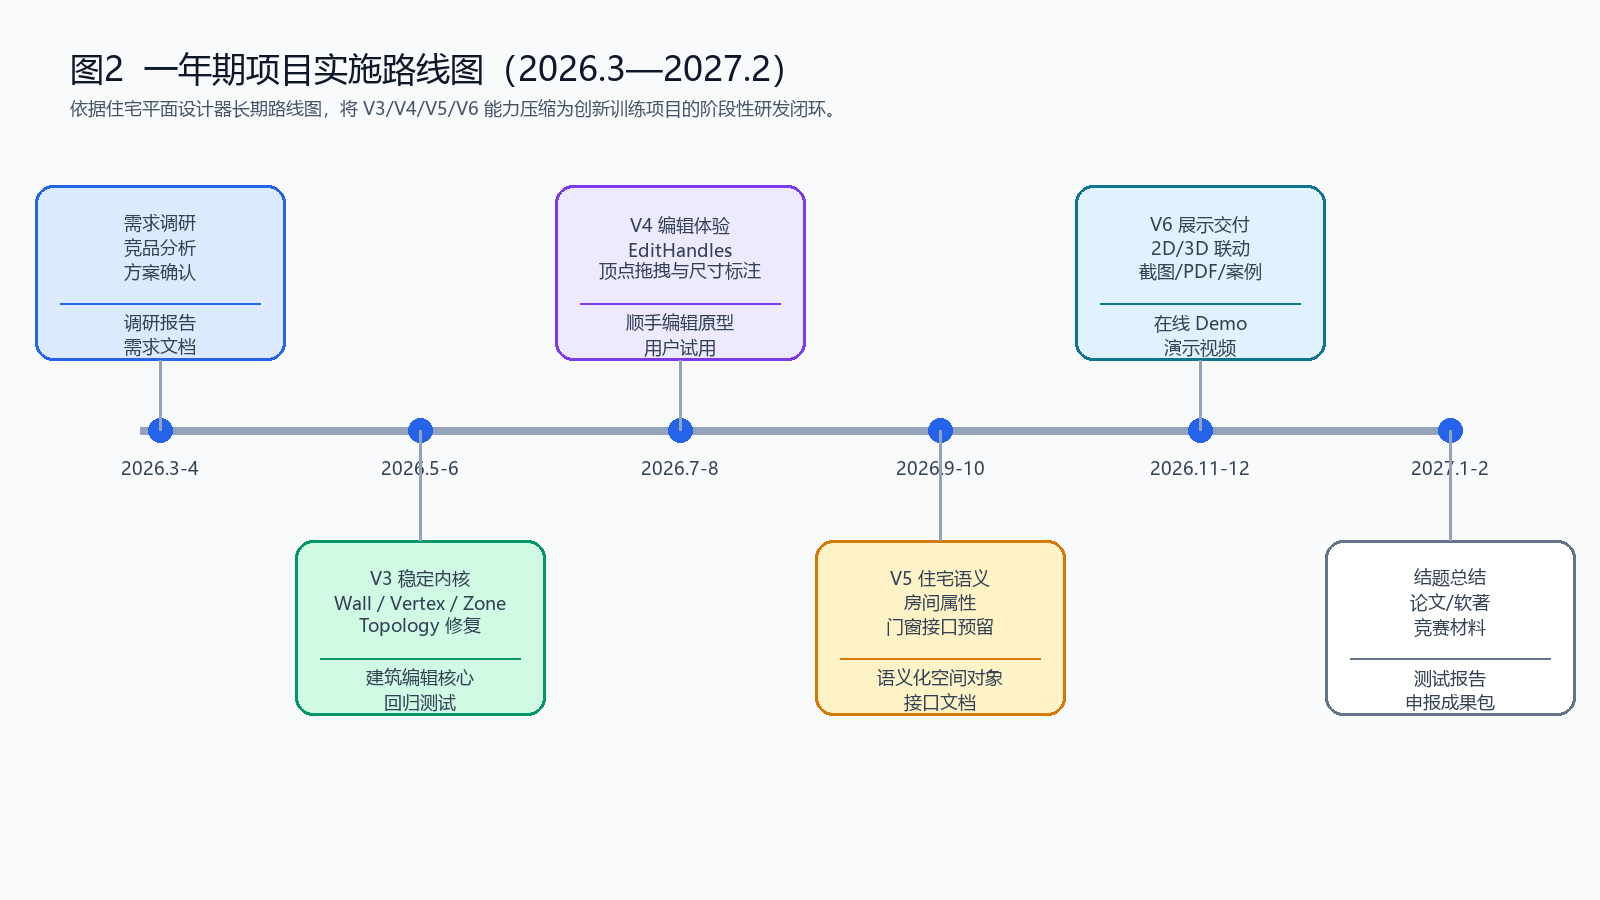
\includegraphics[width=\textwidth]{implementation-roadmap.png}
  \caption{一年期项目实施路线图（2026.3—2027.2）}
\end{figure}

\section{可行性分析}

\subsection{技术可行性}

项目采用的 React、TypeScript、Vite、Three.js、React Three Fiber、Zustand、IndexedDB 等技术均较成熟，能够支撑浏览器端 3D 场景渲染、交互和状态管理。GLB/glTF 已成为 Web 3D 模型常用格式，适合家具模型加载与展示。

项目已有可运行原型，已经实现或具备以下基础能力：

\begin{itemize}
  \item 房间和墙体相关的建筑编辑模块；
  \item 家具模型加载、上传、放置和变换能力；
  \item 墙体透明切换和 3D 场景查看能力；
  \item 本地持久化相关逻辑；
  \item 后端资产服务和数据库迁移基础；
  \item Vitest 单元测试和 Playwright 端到端测试。
\end{itemize}

因此，本项目不是从零开始，而是在已有工程基础上进行系统化研究、完善和验证，技术风险可控。

\subsection{团队可行性}

项目负责人已完成项目原型搭建和核心技术验证，具备前端开发、Web 3D、状态管理和工程测试经验。团队成员可按前端开发、3D 交互、后端资产服务、UI/UX、测试文档等方向分工，形成互补协作。

\subsection{资源可行性}

项目主要依赖开源技术栈和普通开发设备即可完成。部署可采用 GitHub Pages、Vercel、学校服务器或云服务器等方式。模型资源可优先使用开源 GLB 素材和自建测试模型，后续根据经费情况补充商用素材或测试设备。

\subsection{风险与应对}

\begin{longtable}{P{3.8cm}P{4cm}P{7.2cm}}
\toprule
风险 & 影响 & 应对措施 \\
\midrule
\endfirsthead
\toprule
风险 & 影响 & 应对措施 \\
\midrule
\endhead
墙体拓扑编辑复杂度较高 & 可能导致区域识别错误或编辑不稳定 & 采用分阶段路线，优先稳定墙体、顶点、区域核心模型，并补充回归测试 \\
复杂 GLB 模型导致性能下降 & 影响浏览器流畅度 & 限制模型大小，增加加载提示，研究压缩和按需加载策略 \\
普通用户不熟悉 3D 操作 & 使用门槛较高 & 采用建造/装饰两阶段流程，增加可视化反馈和默认视角 \\
本地数据保存失败 & 用户设计内容丢失 & 增加自动保存、异常提示和数据版本管理 \\
项目范围过大 & 影响阶段性成果交付 & 将门窗、多楼层、AI 自动布置等能力放入后续拓展，不纳入首期核心验收 \\
\bottomrule
\end{longtable}

\subsection{应用前景与转化潜力}

本项目以创新训练和技术原型研发为主，不以短期商业化为核心目标，但项目成果具备较明确的后续应用转化空间。面向 C 端用户，平台可服务租房改造、家庭装修预演、家具摆放模拟和家居内容创作等场景，帮助用户在购买家具或改造空间前快速验证布局效果。面向行业服务方，平台可与家具品牌、家装公司、房地产展示和家居电商平台结合，将真实家具模型、样板间方案和在线购买链路接入浏览器端 3D 场景，提高沟通效率和展示转化能力。

在后续迭代中，项目可进一步拓展云端素材库、方案分享链接、AI 自动布局、多端同步和标准户型模板等能力。上述方向既能延续本项目的技术研究价值，也为参加中国国际大学生创新大赛、申请软件著作权以及探索校企合作提供基础。

\section{预期成果}

\begin{enumerate}
  \item \textbf{可运行的 Web 端 3D 家居设计平台 Demo。} 支持浏览器访问，完成房间结构绘制、家具摆放、模型上传和场景保存等核心流程。
  \item \textbf{项目源代码与技术文档。} 形成结构清晰、可持续维护的前后端代码仓库，并整理需求文档、设计文档、接口文档和测试说明。
  \item \textbf{测试与用户体验报告。} 完成单元测试、端到端测试和基础用户体验测试，记录系统性能、可用性和改进方向。
  \item \textbf{论文或技术报告 1 篇。} 论文方向可为《基于 React Three Fiber 的浏览器端轻量化 3D 家居设计平台设计与实现》。
  \item \textbf{软件著作权申请材料 1 项。} 申请名称可暂定为《轻量化 3D 家居设计平台软件 V1.0》。
  \item \textbf{竞赛与展示成果。} 项目可继续参加“互联网+”“挑战杯”等创新创业类竞赛，形成演示视频、答辩 PPT 和项目展示材料。
\end{enumerate}

\section{团队分工}

\begin{longtable}{P{2.8cm}P{4cm}P{8cm}}
\toprule
成员 & 角色 & 主要职责 \\
\midrule
\endfirsthead
\toprule
成员 & 角色 & 主要职责 \\
\midrule
\endhead
刘宇航 & 项目负责人 / 前端架构 & 项目总体统筹、系统架构设计、建筑编辑内核、核心模块集成和结题材料把关 \\
黄灿斌 & 前端开发 & UI 组件、交互流程、编辑器面板和用户操作体验优化 \\
徐峥 & 三维交互与算法 & 三维场景逻辑、模型控制、墙体/区域几何、吸附和约束算法 \\
陶锦昕 & 后端与部署 & 后端资产服务、模型文件管理、数据库、部署与接口联调 \\
肖斯霖 & 测试与文档 & 文献调研、用户需求整理、测试验证、数据汇总和展示材料制作 \\
蒋文萍 & 指导教师 & 研究方向指导、技术路线把关、论文与成果指导 \\
\bottomrule
\end{longtable}

\section{经费预算}

\begin{longtable}{P{1.2cm}P{3.2cm}P{7.5cm}P{2.5cm}}
\toprule
序号 & 类别 & 用途 & 金额 \\
\midrule
\endfirsthead
\toprule
序号 & 类别 & 用途 & 金额 \\
\midrule
\endhead
1 & 实验材料费 & 购买 GLB 家具模型素材、纹理素材、移动存储介质及项目开发测试所需基础材料 & 1200 元 \\
2 & 测试、化验、加工费等 & 云服务器、域名部署、浏览器兼容性测试、模型压缩与样例数据处理等 & 1800 元 \\
3 & 交通、差旅费 & 用户调研、企业或展会交流、校内外答辩和成果展示相关交通支出 & 600 元 \\
4 & 其他 & 文献资料、软件著作权申请、展示海报、演示视频、打印装订和竞赛报名材料制作 & 1400 元 \\
\multicolumn{3}{r}{合计} & 5000 元 \\
\bottomrule
\end{longtable}

\section{参考文献}

\begin{enumerate}[label={[\arabic*]}]
  \item Khronos Group. glTF 2.0 Specification [EB/OL]. \url{https://www.khronos.org/gltf/}.
  \item Three.js Contributors. Three.js Documentation [EB/OL]. \url{https://threejs.org/docs/}.
  \item Poimandres. React Three Fiber Documentation [EB/OL]. \url{https://docs.pmnd.rs/react-three-fiber/}.
  \item WebGL Working Group. WebGL Specification [EB/OL]. \url{https://www.khronos.org/webgl/}.
  \item IndexedDB API Documentation. MDN Web Docs [EB/OL]. \url{https://developer.mozilla.org/}.
  \item Nielsen J. Usability Engineering [M]. Morgan Kaufmann, 1994.
  \item Norman D. The Design of Everyday Things [M]. Basic Books, 2013.
  \item 【补充中文文献】. WebGL 三维可视化系统设计与实现 [J]. 【期刊名称】, 【年份】.
  \item 【补充中文文献】. 基于 Three.js 的室内场景可视化研究 [J]. 【期刊名称】, 【年份】.
  \item 【补充中文文献】. 面向用户体验的室内设计交互系统研究 [J]. 【期刊名称】, 【年份】.
\end{enumerate}

\section{其他说明}

本项目已有明确的工程基础，代码仓库已包含前端编辑器、建筑编辑模块、资产库后端、测试用例和阶段性路线图。后续创新训练将重点围绕“轻量化 Web 3D 家居设计平台”的稳定性、易用性和可验证性开展，而不是单纯堆叠功能。

项目阶段成果将优先保证以下闭环：

\begin{enumerate}
  \item 用户能够在浏览器中快速创建房间结构；
  \item 用户能够上传或选择家具模型并完成布置；
  \item 用户能够保存和恢复自己的设计方案；
  \item 系统能够通过自动化测试验证关键交互；
  \item 项目能够以 Demo、文档、论文和软著形式形成可提交成果。
\end{enumerate}

\end{document}
